
%%%%%%%%%%%%%%%%%%%%%%%%%%%%%%%%%%%%%%%%%%%%%%%%%%%%%%%%%%%%%%%%%%%
\newcommand{\largeur}{0.5}
\newcommand{\hauteur}{1.5}
\newcommand{\rayon}{0.075cm}
\newcommand{\ytext}{-1}
\newcommand{\ytexth}{3*\hauteur+2.5}
\newcommand{\dlayer}[3]{ \draw[fill=#3] (#1,#2) rectangle (#1+\largeur,#2+\hauteur); %
  \foreach \y in {0.25,0.5,...,1.25}{ \draw[fill=black] (#1+\largeur/2,#2+\y) circle (\rayon);};%
}
\newcommand{\greenhc}{\color{green!50!black}}
\newcommand{\hiddenl}{\greenhc\seq{h}_t}

%%%%%%%%%%%%%%%%%%%%%%%%%%%%%%%%%%%%%%%%%%%%%%%%%%%%%%%%%%%%%%%%%%%


\begin{frame}{Sequence processing}
  \begin{block}{Sequence generation model}
    $$
    P(\wsseq{1}{L}) = P(\ws_1, \ws_2, ... \ws_L) = \prod_{i=1}^L P(\ws_i | \wsseq{1}{i-1}),\ \ \forall i , \ws_i \in \vocab
    $$
    with the \textbf{\ngram assumption} (convolution):
    $$
    P(\wsseq{1}{L}) = \prod_{i=1}^L P(\ws_i | \wsseq{i-n+1}{i-1}),\ \ \forall i , \ws_i \in \vocab,
    $$
    in the \textbf{recurrent} way 
    $$ P(\ws_i | \wsseq{1}{i-1})$$
  \end{block}
  \begin{block}{Sequence representation}
    \begin{center}
      \begin{tikzpicture}
        %%%%%%%%%%%%%%%%%%%%% 
        \node[anchor=east,draw=gray,text width=0.3\textwidth,align=center] (review) at
        (0,0) {\cga~\cgt~\cgc~\cgg~\cga~\cgt~\cgc~\cgg\\$\cdots$~\cgg~\cgt~\cga~\cga~\cgt~\cgc~\cgg};
        %%%%%%%%%%%%%%%%%%%%% 
        \node[anchor=west] (txt) at (0.1,0) {$: \ \x \in \real^{\nfeats} \ \longrightarrow \ \class \in\{0, 1\}$};
      \end{tikzpicture}
    \end{center}
  \end{block}
\end{frame}

\begin{frame}{Recurrent Cell}
  \begin{columns}
    \begin{column}{0.5\textwidth}
      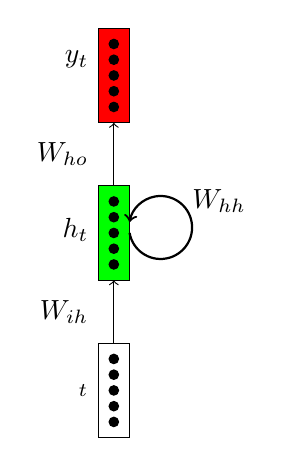
\begin{tikzpicture}[scale=0.8]
        % words embeddings
        \dlayer{0}{0}{white};
        % hidden layers
        \dlayer{0}{\hauteur+1}{green};
        % output layers
        \dlayer{0}{2*\hauteur+2}{red};
        % links from embeddings to hidden layers
        \draw[->] (\largeur/2,0+\hauteur) -- (\largeur/2,\hauteur+1);%
        % links from hidden layers to output
        \draw[->] (\largeur/2,2*\hauteur+1) --
        (\largeur/2,2*\hauteur+2);%
        \draw[->,thick] (\largeur,1.5*\hauteur+1) arc (10:350:-0.5);
        % Put parameters
        \node[anchor=east] at (-0,\hauteur/2){$\x_t$};%
        \node[anchor=east] at (-0,4*\hauteur){$\seq{y}_t$};%
        \node[anchor=east] at (-0,2.2*\hauteur){$\seq{h}_t$};%
        \node[anchor=east] at (-0,\hauteur+0.5){$\seq{W}_{ih}$};%
        \node[anchor=east] at (-0,2*\hauteur+1.5){$\seq{W}_{ho}$};%
        \node[anchor=east] at
        (4*\largeur+0.5,1.5*\hauteur+1.5){$\seq{W}_{hh}$};%
      \end{tikzpicture}
    \end{column}
    \begin{column}{0.5\textwidth}
      A dynamic system, at time $t$:
      \begin{itemize}
      \item maintains a hidden representation, the internal state:  $\seq{h}_t$
      \item Updated with the observation of $\x_t$  and the previous state $\seq{h}_{t-1}$
      \item The prediction $\seq{y}_t$ depends on the internal state ($\seq{h}_t$)
      \item For a language model, $\x_t$ comes from word embeddings
      \end{itemize}
    \end{column}
  \end{columns}
  \begin{center}\vfill
    The same parameter set is shared across time steps
  \end{center}
\end{frame}


%%%%%%%%%%%%%%%%%%%%%%%%%%%%%%%%%%%%%% 
\begin{frame}{Recurrent network sequence model}
  \framesubtitle{Unfolding the structure: a deep-network}
  \begin{columns}
    \begin{column}{0.5\textwidth}
      \begin{center}
        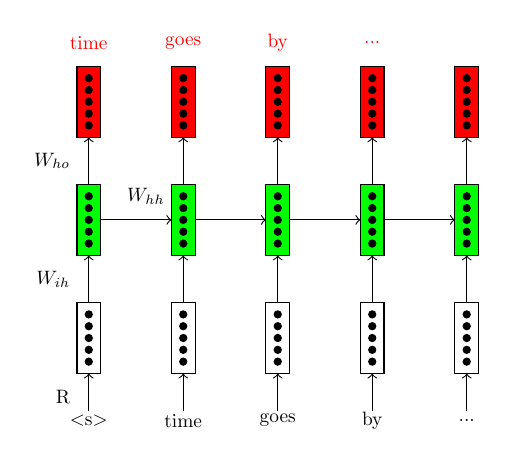
\begin{tikzpicture}[scale=0.6,every node/.style={scale=0.7}]
          \node[anchor=center] (time) at (0+\largeur/2,\ytext)
          {$<$s$>$}; \node[anchor=center] (goes) at
          (2+\largeur/2,\ytext) {time}; \node[anchor=center] (by) at
          (4+\largeur/2,\ytext) {goes}; \node[anchor=center] (so) at
          (6+\largeur/2,\ytext) {by}; \node[anchor=center] (dots) at
          (8+\largeur/2,\ytext) {...};
          % words embeddings
          \foreach \x in {0,2,...,8}{\dlayer{\x}{0}{white}};
          % hidden layers
          \foreach \x in {0,2,...,8}{\dlayer{\x}{\hauteur+1}{green}};
          % output layers
          \foreach \x in {0,2,...,8}{\dlayer{\x}{2*\hauteur+2}{red}};
          % links from text to embeddings
          \foreach \x in {0,2,...,8}{\draw[->]
            (\x+\largeur/2,\ytext+0.2) -- (\x+\largeur/2,0);};
          % links from embeddings to hidden layers
          \foreach \x in {0,2,...,8}{\draw[->]
            (\x+\largeur/2,0+\hauteur) --
            (\x+\largeur/2,\hauteur+1);};
          % links between hidden layers
          \foreach \x in {0,2,...,6}{\draw[->]
            (\x+\largeur,1.5*\hauteur+1) -- (\x+2,1.5*\hauteur+1);};
          % links from hidden layers to output
          \foreach \x in {0,2,...,8}{\draw[->]
            (\x+\largeur/2,2*\hauteur+1) --
            (\x+\largeur/2,2*\hauteur+2);}; {\color{red}
            \node[anchor=center] (time) at (0+\largeur/2,\ytexth)
            {time}; \node[anchor=center] (goes) at
            (2+\largeur/2,\ytexth) {goes}; \node[anchor=center] (by)
            at (4+\largeur/2,\ytexth) {by}; \node[anchor=center] (so)
            at (6+\largeur/2,\ytexth) {...};}
          % Put parameters
          \node[anchor=east] at (-0,\ytext+0.5){\seq{R}};
          \node[anchor=east] at (-0,\hauteur+0.5){$\seq{W}_{ih}$};
          \node[anchor=east] at (-0,2*\hauteur+1.5){$\seq{W}_{ho}$};
          \node[anchor=east] at
          (4*\largeur,1.5*\hauteur+1.5){$\seq{W}_{hh}$};
          % Legend:
          % \node[anchor=east] (sent) at (-1,\ytext) {\textbf{Input
          % sequence: }};
          % \node[anchor=east] (sent) at (-1,\ytext+0.5)
          % {\textbf{embeddings: }};
        \end{tikzpicture}
      \end{center}
    \end{column}
    \begin{column}{0.5\textwidth}
      At each step $t$
      \begin{itemize}
      \item Read the word $w_t \rightarrow \x_t$ from $\seq{R}$
      \item Update the hidden state $\seq{h}_t = f(\seq{W}_{ih} \x_t + \seq{W_{hh}\seq{h}_{t-1}})$
      \item The word at $t+1$ can be predicted from $\seq{h}_t$:
        $$
        \seq{y}_t = g(\seq{W}_{ho} \seq{h}_t)
        $$
      \item $g$ is the softmax function over the vocabulary
      \end{itemize}
    \end{column}
  \end{columns}
\end{frame}



%%%%%%%%%%%%%%%%%%%%%%%%%%%%%%%%%%%%%% 
\begin{frame}{Training recurrent language model}
  \begin{block}{Training algorithm}
    Back-Propagation through time or
    BPTT\\\cite{Rumelhart86BPTT,Mikolov11Extension}:\\
    \begin{itemize}
    \item for each step $t$
      \begin{itemize}
      \item compute the loss gradient
      \item Back-Propagation through the unfolded structure
      \end{itemize}
    \end{itemize}
  \end{block}
  \begin{block}{Inference}
    \begin{itemize}
    \item Cannot be easily integrated to conventional approaches (ASR, SMT, ... )
    \item A powerful device for end-to-end system
    \end{itemize}
  \end{block}
\end{frame}

%%%%%%%%%%%%%%%%%%%%%%%%%%%%%%%%%%%%%% 
\begin{frame}{Training recurrent language model - 2}
  \begin{center}
        \begin{tikzpicture}[scale=0.6,every node/.style={scale=0.7}]
          \node[anchor=center] (time) at (0+\largeur/2,\ytext)
          {$<$s$>$}; \node[anchor=center] (goes) at
          (2+\largeur/2,\ytext) {time}; \node[anchor=center] (by) at
          (4+\largeur/2,\ytext) {goes}; \node[anchor=center] (so) at
          (6+\largeur/2,\ytext) {by}; \node[anchor=center] (dots) at
          (8+\largeur/2,\ytext) {...};
          % words embeddings
          \foreach \x in {0,2,...,8}{\dlayer{\x}{0}{white}};
          % hidden layers
          \foreach \x in {0,2,...,8}{\dlayer{\x}{\hauteur+1}{green}};
          % output layers
          \foreach \x in {0,2,...,8}{\dlayer{\x}{2*\hauteur+2}{red}};
          % links from text to embeddings
          \foreach \x in {0,2,...,8}{\draw[->]
            (\x+\largeur/2,\ytext+0.2) -- (\x+\largeur/2,0);};
          % links from embeddings to hidden layers
          \foreach \x in {0,2,...,8}{\draw[->]
            (\x+\largeur/2,0+\hauteur) --
            (\x+\largeur/2,\hauteur+1);};
          % links between hidden layers
          \foreach \x in {0,2,...,6}{\draw[->]
            (\x+\largeur,1.5*\hauteur+1) -- (\x+2,1.5*\hauteur+1);};
          % links from hidden layers to output
          \foreach \x in {0,2,...,8}{\draw[->]
            (\x+\largeur/2,2*\hauteur+1) --
            (\x+\largeur/2,2*\hauteur+2);}; 
          %%% output words 
          {\color{red}
            \node[anchor=center] (time) at (0+\largeur/2,\ytexth)
            {time}; \node[anchor=center] (goes) at
            (2+\largeur/2,\ytexth) {goes}; \node[anchor=center] (by)
            at (4+\largeur/2,\ytexth) {by}; \node[anchor=center] (so)
            at (6+\largeur/2,\ytexth) {...};
          }
          %%%% loss
          {\color{red}
            \node[anchor=center] (ltime) at (0+\largeur/2,\ytexth+0.5)
            {$\ploss_{\params}$(time)}; 
            
            \node[anchor=center] (lgoes) at
            (2+\largeur/2,\ytexth+0.5) {$\ploss_{\params}$(goes)}; 

            \node[anchor=center] (lby)
            at (4+\largeur/2,\ytexth+0.5) {$\ploss_{\params}$(by)}; 
            
            \node[anchor=center] (lso)
            at (6+\largeur/2,\ytexth+0.5) {$\ploss_{\params}$(so)};


            \node[anchor=center] (lfin)
            at (8+\largeur/2,\ytexth+0.5) {$\ploss_{\params}$(...)};
          }
          
          \node[anchor=center,red] (loss)
            at (4+\largeur/2,\ytexth+2) {$\sum_i \ploss_{\params} (w_i)$}; 
            
          \draw[->,red] (ltime) -- (loss);
          \draw[->,red] (lgoes) -- (loss);
          \draw[->,red] (lby) -- (loss);
          \draw[->,red] (lso) -- (loss);
          \draw[->,red] (lfin) -- (loss);
          % Put parameters
          \node[anchor=east] at (-0,\ytext+0.5){\seq{R}};
          \node[anchor=east] at (-0,\hauteur+0.5){$\seq{W}_{ih}$};
          \node[anchor=east] at (-0,2*\hauteur+1.5){$\seq{W}_{ho}$};
          \node[anchor=east] at
          (4*\largeur,1.5*\hauteur+1.5){$\seq{W}_{hh}$};
          % Legend:
          % \node[anchor=east] (sent) at (-1,\ytext) {\textbf{Input
          % sequence: }};
          % \node[anchor=east] (sent) at (-1,\ytext+0.5)
          % {\textbf{embeddings: }};
        \end{tikzpicture}
      \end{center}
\end{frame}



%%%%%%%%%%%%%%%%%%%%%%%%%%%%%%%%%%%%%% 

\begin{frame}{Mini-batching for RNN}
  \begin{center}
    Mini-batching makes things much faster!
  \end{center}
  \begin{block}{Mini-batch}
    \begin{itemize}
    \item Add a dimension to your input example $\x$
    \item Forward propagation of the whole mini-batch at a time
    \item Compute the loss and back-propagation
    \end{itemize}
  \end{block}

  \begin{block}{But}
    \begin{itemize}
    \item mini-batching in RNNs is harder than in feed-forward
      networks
    \item Each word depends on the previous word
    \item Sequences are of various length
    \end{itemize}
  \end{block}

\end{frame}

\begin{frame}{Batching / Padding / Masking}
  \begin{center}
        \includegraphics[width=0.8\textwidth]{../figs/batch_mask}\\
 {  \scriptsize Figure from G. Neubig}
  \end{center}
\end{frame}


%%%%%%%%%%%%%%%%%%%%%%%%%%%%%%%%%%%%%% 
\begin{frame}{Short term memory}
  \begin{columns}
    \begin{column}{0.5\textwidth}
      \begin{center}
        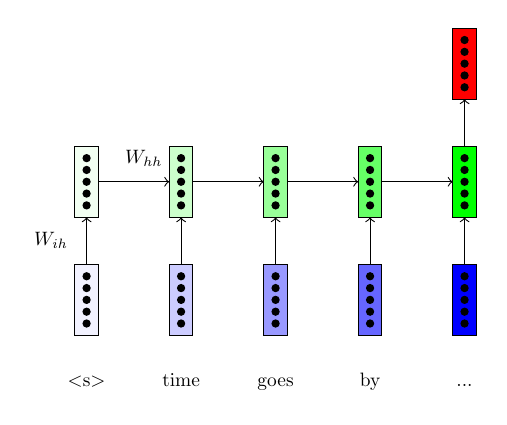
\begin{tikzpicture}[scale=0.6,every node/.style={scale=0.7}]
          \node[anchor=mid] (time) at (0+\largeur/2,\ytext)
          {$<$s$>$}; \node[anchor=mid] (goes) at
          (2+\largeur/2,\ytext) {time}; \node[anchor=mid] (by) at
          (4+\largeur/2,\ytext) {goes}; \node[anchor=mid] (so) at
          (6+\largeur/2,\ytext) {by}; \node[anchor=mid] (dots) at
          (8+\largeur/2,\ytext) {...};
          % words embeddings
          \dlayer{0}{0}{blue!5};
          \dlayer{2}{0}{blue!20};
          \dlayer{4}{0}{blue!40};
          \dlayer{6}{0}{blue!60};
          \dlayer{8}{0}{blue};

          % hidden layers
          \dlayer{0}{\hauteur+1}{green!5};
          \dlayer{2}{\hauteur+1}{green!20};
          \dlayer{4}{\hauteur+1}{green!40};
          \dlayer{6}{\hauteur+1}{green!60};
          \dlayer{8}{\hauteur+1}{green};
          % output layers
          \foreach \x in {8}{\dlayer{\x}{2*\hauteur+2}{red}};
          % links from embeddings to hidden layers
          \foreach \x in {0,2,...,8}{\draw[->]
            (\x+\largeur/2,0+\hauteur) --
            (\x+\largeur/2,\hauteur+1);};
          % links between hidden layers
          \foreach \x in {0,2,...,6}{\draw[->]
            (\x+\largeur,1.5*\hauteur+1) -- (\x+2,1.5*\hauteur+1);};
          % Put parameters
          \node[anchor=east] at (-0,\hauteur+0.5){$\seq{W}_{ih}$};
          % \node[anchor=east] at (-0,2*\hauteur+1.5){$\seq{W}_{ho}$};
          \node[anchor=east] at
          (4*\largeur,1.5*\hauteur+1.5){$\seq{W}_{hh}$};
          % links from hidden layers to output
          \foreach \x in {8}{\draw[->]
            (\x+\largeur/2,2*\hauteur+1) --
            (\x+\largeur/2,2*\hauteur+2);}; 
        \end{tikzpicture}
      \end{center}
    \end{column}
    \begin{column}{0.5\textwidth}
      During inference : 
      \begin{itemize}
      \item With the distance, the influence of observations reduces
      \item The memory is limited
      \item No way to keep/skip information
      \end{itemize}
    \end{column}
  \end{columns}
\end{frame}


\begin{frame}{Vanishing gradient issue}
  \begin{columns}
    \begin{column}{0.5\textwidth}
      \begin{center}
        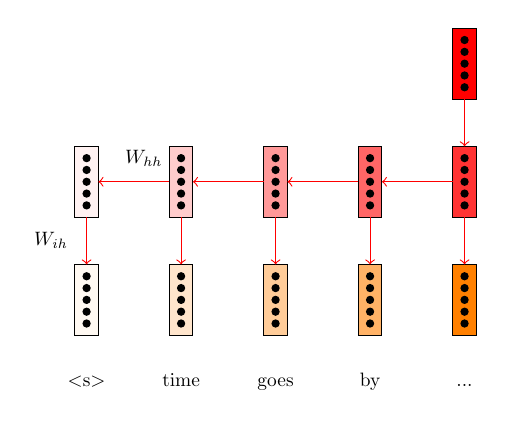
\begin{tikzpicture}[scale=0.6,every node/.style={scale=0.7}]
          \node[anchor=mid] (time) at (0+\largeur/2,\ytext)
          {$<$s$>$}; \node[anchor=mid] (goes) at
          (2+\largeur/2,\ytext) {time}; \node[anchor=mid] (by) at
          (4+\largeur/2,\ytext) {goes}; \node[anchor=mid] (so) at
          (6+\largeur/2,\ytext) {by}; \node[anchor=mid] (dots) at
          (8+\largeur/2,\ytext) {...};
          % words embeddings
          % words embeddings
          \dlayer{0}{0}{orange!5};
          \dlayer{2}{0}{orange!20};
          \dlayer{4}{0}{orange!40};
          \dlayer{6}{0}{orange!60};
          \dlayer{8}{0}{orange};
          % hidden layers
          \dlayer{0}{\hauteur+1}{red!5};
          \dlayer{2}{\hauteur+1}{red!20};
          \dlayer{4}{\hauteur+1}{red!40};
          \dlayer{6}{\hauteur+1}{red!60};
          \dlayer{8}{\hauteur+1}{red!80};
          % output layers
          \foreach \x in {8}{\dlayer{\x}{2*\hauteur+2}{red}};
          % links from embeddings to hidden layers
          \foreach \x in {0,2,...,8}{\draw[<-,red]
            (\x+\largeur/2,0+\hauteur) --
            (\x+\largeur/2,\hauteur+1);};
          % links between hidden layers
          \foreach \x in {0,2,...,6}{\draw[<-,red]
            (\x+\largeur,1.5*\hauteur+1) -- (\x+2,1.5*\hauteur+1);};
          % Put parameters
          \node[anchor=east] at (-0,\hauteur+0.5){$\seq{W}_{ih}$};
          % \node[anchor=east] at (-0,2*\hauteur+1.5){$\seq{W}_{ho}$};
          \node[anchor=east] at
          (4*\largeur,1.5*\hauteur+1.5){$\seq{W}_{hh}$};
          % links from hidden layers to output
          \foreach \x in {8}{\draw[<-,red]
            (\x+\largeur/2,2*\hauteur+1) --
            (\x+\largeur/2,2*\hauteur+2);}; 
        \end{tikzpicture}
      \end{center}
    \end{column}
    \begin{column}{0.5\textwidth}
      During training: 
      \begin{itemize}
      \item The gradient diminishes at each backward step
      \item No long term propagation of the gradient
      \end{itemize}
    \end{column}
  \end{columns}
\end{frame}






%%%%%%%%%%%%%%%%%%%%%%%%%%%%%%%%%%%%%% 
\begin{frame}{The Problem of Long-Term Dependencies}
    \begin{center}
        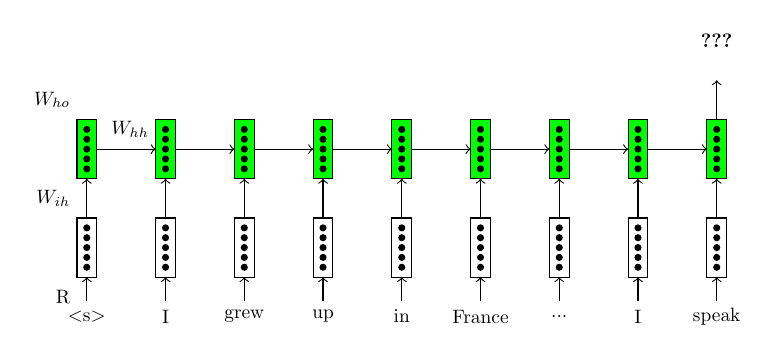
\begin{tikzpicture}[scale=0.5,every node/.style={scale=0.7}]
          \node[anchor=center] (time) at (0+\largeur/2,\ytext){$<$s$>$};
          \node[anchor=center] (goes) at (2+\largeur/2,\ytext) {I};
          \node[anchor=center] (by) at (4+\largeur/2,\ytext) {grew};
          \node[anchor=center] (so) at (6+\largeur/2,\ytext) {up};
          \node[anchor=center] (so) at (8+\largeur/2,\ytext) {in};
          \node[anchor=center] (so) at (10+\largeur/2,\ytext) {France};
          \node[anchor=center] (so) at (12+\largeur/2,\ytext) {...};
          \node[anchor=center] (so) at (14+\largeur/2,\ytext) {I};
          \node[anchor=center] (so) at (16+\largeur/2,\ytext) {speak};
          % words embeddings
          \foreach \x in {0,2,...,16}{\dlayer{\x}{0}{white}};
          % hidden layers
          \foreach \x in {0,2,...,16}{\dlayer{\x}{\hauteur+1}{green}};
          % output layers
          %\foreach \x in {0,2,...,8}{\dlayer{\x}{2*\hauteur+2}{red}};
          % links from text to embeddings
          \foreach \x in {0,2,...,16}{\draw[->]
            (\x+\largeur/2,\ytext+0.4) -- (\x+\largeur/2,0);};
          % links from embeddings to hidden layers
          \foreach \x in {0,2,...,16}{\draw[->]
            (\x+\largeur/2,0+\hauteur) --
            (\x+\largeur/2,\hauteur+1);};
          % links between hidden layers
          \foreach \x in {0,2,...,14}{\draw[->]
            (\x+\largeur,1.5*\hauteur+1) -- (\x+2,1.5*\hauteur+1);};
          % links from hidden layers to output
          \draw[->](16+\largeur/2,2*\hauteur+1) --
            (16+\largeur/2,2*\hauteur+2);
          % output 
          {\node[anchor=center] (time) at (16+\largeur/2,\ytexth-1)
            {\bf ???}; }
          % Put parameters
          \node[anchor=east] at (-0,\ytext+0.5){\seq{R}};
          \node[anchor=east] at (-0,\hauteur+0.5){$\seq{W}_{ih}$};
          \node[anchor=east] at (-0,2*\hauteur+1.5){$\seq{W}_{ho}$};
          \node[anchor=east] at
          (4*\largeur,1.5*\hauteur+1.5){$\seq{W}_{hh}$};
        \end{tikzpicture}
      \end{center}
  \begin{itemize}
  \item Recent observations hide the older ones~\cite{Bengio94Long}
  \item The vanishing (exploding) gradient is a real issue~\cite{Pascanu13Difficulty}
  \end{itemize}
\end{frame}



%%%%%%%%%%%%%%%%%%%%%%%%%%%%%%%%%%%%%% 
\begin{frame}{Solutions}
  \begin{block}{Improved optimization}
    \begin{itemize}
    \item Gradient clipping~\cite{Pascanu13Difficulty} 
    \item Hessian-Free optimzation~\cite{Martens12HF} or natural gradient~\cite{Desjardins13Natural,Ollivier15Riemannian}
    \end{itemize}
  \end{block}
  \begin{block}{Modified unit}
    A recurrent network should be able to mitigate the observations \textit{vs} its internal state: 
    \begin{itemize}
    \item LSTM or Long-Short-Term-Memory cell~\cite{Hochreiter97LSTM,Graves09Offline}
    \item  Gated Recurrent Unit or GRU~\cite{Cho14Learning}
    \end{itemize}
  \end{block}
\end{frame}


%%%%%%%%%%%%%%%%%%%%%%%%%%%%%%%%%%%%%% 
\begin{frame}{Gradient clipping}
A simple and efficient trick\\
Given a threshold $\gamma$, before each update: 
\begin{itemize}
\item Compute the norm of the gradient (at each time step) :   $||\pgrad{\params}||$
\item If  $ ||\pgrad{\params}|| > \gamma$: 
$$ \pgrad{\params} \leftarrow \frac{\gamma}{||\pgrad{\params}|| } \pgrad{\params} 
$$
\end{itemize}
\end{frame}
%%%%%%%%%%%%%%%%%%%%%%%%%%%%%%%%%%%%%% 

\begin{frame}{Sentence encoder: the bi-recurrent solution}
  \begin{columns}
    \begin{column}{0.5\textwidth}
      \begin{center}
        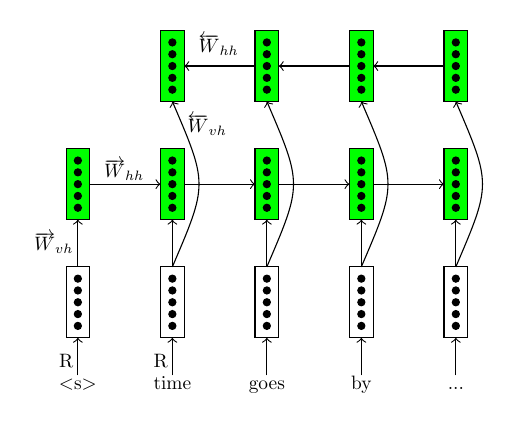
\begin{tikzpicture}[scale=0.6,every node/.style={scale=0.7}]
          \node[anchor=mid] (time) at (0+\largeur/2,\ytext)  {$<$s$>$}; 
          \node[anchor=mid] (goes) at   (2+\largeur/2,\ytext) {time}; 
          \node[anchor=mid] (by) at
          (4+\largeur/2,\ytext) {goes}; 
          \node[anchor=mid] (so) at
          (6+\largeur/2,\ytext) {by}; 
          \node[anchor=mid] (dots) at
          (8+\largeur/2,\ytext) {...};
          % words embeddings
          \foreach \x in {0,2,...,8}{\dlayer{\x}{0}{white}};
          % hidden layers
          \foreach \x in {0,2,...,8}{\dlayer{\x}{\hauteur+1}{green}};
          % 2nd stage of hidden layers
          \foreach \x in {2,4,...,8}{\dlayer{\x}{2*\hauteur+2}{green}};
          % links from text to embeddings
          \foreach \x in {0,2,...,8}{\draw[->]
            (\x+\largeur/2,\ytext+0.2) -- (\x+\largeur/2,0);};
          % links from embeddings to hidden layers
          \foreach \x in {0,2,...,8}{\draw[->]
            (\x+\largeur/2,0+\hauteur) --
            (\x+\largeur/2,\hauteur+1);};
         % links between hidden layers (first stage)
          \foreach \x in {0,2,...,6}{\draw[->]
            (\x+\largeur,1.5*\hauteur+1) -- (\x+2,1.5*\hauteur+1);};
         % links between hidden layers (2nd stage)
          \foreach \x in {2,4,...,6}{\draw[<-]
            (\x+\largeur,3*\hauteur+1.25) -- (\x+2,3*\hauteur+1.25);};
          % links from embeddings to  hidden layers 2nd stage
          \foreach \x in {2,4,...,8}{
            \draw[->]  (\x+\largeur/2,0+\hauteur).. controls (\x+2*\largeur,0+1.5*\hauteur+1) ..
            (\x+\largeur/2,2*\hauteur+2);};
      
          % Put parameters
          \node[anchor=east] at (0.3,\ytext+0.5){\seq{R}};
          \node[anchor=east] at (2.3,\ytext+0.5){\seq{R}};
          \node[anchor=east] at (0.3,\hauteur+0.5){$\overrightarrow{\seq{W}}_{vh}$};
          \node[anchor=east] at (3.55,2*\hauteur+1.5){$\overleftarrow{\seq{W}}_{vh}$};
          \node[anchor=east] at
          (4*\largeur-0.2,1.5*\hauteur+1.3){$\overrightarrow{\seq{W}}_{hh}$};
          \node[anchor=east] at
          (2+4*\largeur-0.2,3*\hauteur+1.7){$\overleftarrow{\seq{W}}_{hh}$};
        \end{tikzpicture}
      \end{center}
    \end{column}
    \begin{column}{0.5\textwidth}
      A each step $t$, from left to right
      \begin{itemize}
      \item $w_t \rightarrow \inp_t$
      \item ${\greenhc\overrightarrow{\seq{h}}_t } = f(\overrightarrow{\seq{W}}_{vh} \inp_t + \overrightarrow{\seq{W}}_{hh}\overrightarrow{\seq{h}}_{t-1})$
      \end{itemize}
      A each step $t$, from right to left
      \begin{itemize}
      \item $w_t \rightarrow \inp_t$
      \item ${\greenhc\overleftarrow{\seq{h}}_t} = f(\overleftarrow{\seq{W}}_{vh} \inp_t + \overleftarrow{\seq{W}}_{hh}\overleftarrow{\seq{h}}_{t-1})$
      \end{itemize}
    \end{column}
  \end{columns}
  \begin{center}
\textbf{    $[ {\greenhc\overrightarrow{\seq{h}}_t} ;
  {\greenhc\overleftarrow{\seq{h}}_t}]$ : contextualized
  representation of  $\ws_t$}
  \end{center}
\end{frame}

\begin{frame}{Sequence representation}
    \begin{center}
        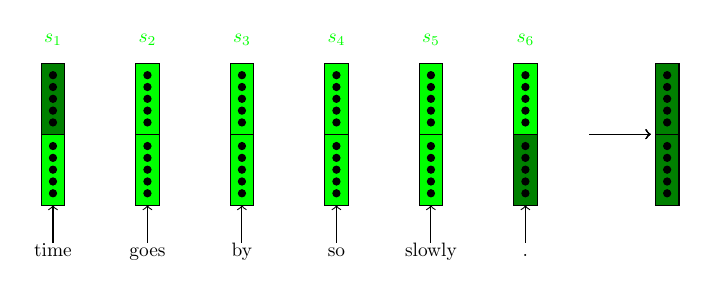
\begin{tikzpicture}[scale=0.6,every node/.style={scale=0.7}]
          \node[anchor=mid] (goes) at   (2+\largeur/2,\ytext) {time}; 
          \node[anchor=mid] (by) at  (4+\largeur/2,\ytext) {goes}; 
          \node[anchor=mid] (so) at  (6+\largeur/2,\ytext) {by}; 
          \node[anchor=mid] (dots) at  (8+\largeur/2,\ytext) {so};
          \node[anchor=mid] (dots) at  (10+\largeur/2,\ytext) {slowly};
          \node[anchor=mid] (dots) at  (12+\largeur/2,\ytext) {.};
          % hidden layers
          \foreach \x in {2,4,...,12}{\dlayer{\x}{0}{green}};
          % 2nd stage of hidden layers
          \foreach \x in {2,4,...,12}{\dlayer{\x}{\hauteur}{green}};
          % links from text to embeddings
          \foreach \x in {2,4,...,12}{\draw[->]
            (\x+\largeur/2,\ytext+0.2) -- (\x+\largeur/2,0);};
          % name the representation 
          \foreach \x in {1,2,...,6}{
          \node[anchor=center,green] (s1) at (2*\x+\largeur/2,\ytext+3*\hauteur) {$\seq{s}_{{\x}}$}; 

          %%% 
          \only<2>{
            \foreach \x in {12}{\dlayer{\x}{0}{green!50!black}};
            \foreach \x in {2}{\dlayer{\x}{\hauteur}{green!50!black}};
            \dlayer{15}{0}{green!50!black};
            \dlayer{15}{\hauteur}{green!50!black};
            \draw[black,->] (13.1+\largeur,\hauteur) -> (15-0.1,\hauteur);
          }
          };

        \end{tikzpicture}
      \end{center}  
      \begin{itemize}
      \item A bi-recurrent encoder
      \item Each observation is associated to a vector: a
        contextualised representation $\greenhc \seq{s_t} $
      \end{itemize}
\end{frame}
